%%%%Use this as a filler to get the template working
%%Introduction
\chapter{Analysis}
This chapter will present the results of a search for Higgs boson pair production where one Higgs boson decays via ${H\rightarrow b\overline{b}}$ and the other via ${H\rightarrow WW^{*}}$. The ${WW^{*}}$ system decays into ${l\nu qq}$ (where ${l}$ is either an electron or a muon), with the small contamination from the leptonic ${\tau}$ decays is not explicitly vetoed in the analysis. The Higgs boson decay modes chosen for this analysis are a compromise between signal efficiency and background reduction. The ${H\rightarrow WW^{*}}$ branching ratio of approximately 25\% is the second largest after ${H\rightarrow b\overline{b}}$ (approximately 58\%). The 1-lepton final state gives a strong discriminator against multijet background. The dominant backgrounds are \ttbar{} production, W bosons produced in association with jets (W+jets), and multijet events where a jet is misidentified as a lepton. There are smaller background  contributions from single top-quark production, Z bosons produced in association with jets (Z+jets), and diboson production.\newline

\begin{figure}[h]
\begin{center}
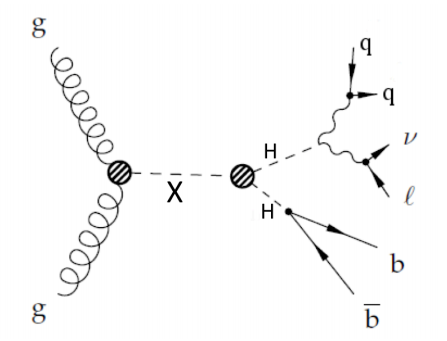
\includegraphics[scale=0.65]{figures/res_prod}
\caption{Schematic diagram of resonant Higgs boson pair production with the subsequent Higgs and W boson
decays.}
\end{center}
\label{fig:res}
\end{figure}

\indent This analysis sets limits on both SM Higgs boson pair production and on resonant production. Both production methods are discussed in detail in chapter \ref{chap:dihiggs}. Figure ~\ref{fig:res} shows a Feynman diagram of resonant production of the Higgs boson pairs with the subsequent decays ${H\rightarrow WW^{*}}$ and ${H\rightarrow b\overline{b}}$.

\section{Analysis Overview}
Two complementary techniques are used to reconstruct the Higgs boson candidates that decays into two b-quarks. Both techniques use the ${\textrm{anti-}k_{t}}$ jet algorithm but with different radius parameters. The first technique uses jets with a radius parameter R = 0.4 and it is used when each b-quark from the ${H\rightarrow b\overline{b}}$ decay can be reconstructed as a distinct b-jet. This is referred to as the ``resolved analysis". The second technique uses jets with a radius parameter R = 1.0, also know as fatjets, and is used when the b-quarks cannot be reconstructed as two distinct b-jets. Instead the Higgs boson candidate is identified as the single fatjet. This technique is referred to as the ``boosted analysis". In both analyses, the jets from the hadronically decaying W boson are reconstructed as ${\textrm{anti-}k_{t}}$ jets with radius parameter R = 0.4. The non-resonant, SM production, search uses the resolved analysis exclusively, while the resonant analysis is performed using either the resolved or boosted analysis technique with the most sensitive technique chosen for each particular model and HH mass being tested.
\section{Data and Monte Carlo Samples}
\subsection{Data}
\indent The analysis presented uses the full proton-proton collision dataset collected in 2015 and 2016 as th center-of-mass energy of 13 TeV passing data quality checks requiring good conditions of all sub-detectors. The data that are currently used correspond to an integrated luminosity of 36.1 fb\textsuperscript{-1} (3.2 fb\textsuperscript{-1} from 2015 plus 32.8 fb\textsuperscript{-1} from 2016)\footnote{The following GoodRunLists (GRL) are used:\\  
data15\_13TeV.periodAllYear\_DetStatus-v79-repro20-02\_DQDefects-00-02-02\_PHYS\_StandardGRL\_All\_Good\_25ns.xml\\
and\\
data16\_13TeV.periodAllYear\_DetStatus-v88-pro20-21\_DQDefects-00-02-04\_PHYS\_StandardGRL\_All\_Good\_25ns.xml.\\
The GRLs were retrieved from the \href{https://twiki.cern.ch/twiki/bin/view/AtlasProtected/GoodRunListsForAnalysisRun2}{GoodRunListsForAnalysisRun2 twiki}}.

. 
\subsection{Monte Carlo Samples}
With the exception of the QCD multijet background described in~\ref{sec:multijet}, MC simulated events are used to estimate SM
backgrounds and the signal acceptances. Table~\ref{tabular:mc_samples} summarizes the MC samples
used for background estimation.

\begin{table}[!htb]
\begin{center}
\begin{tabular}{|l|c|c|}
  \hline
 Process & Generator       & $\sigma\times\text{BR}$ [pb]  \\ 
\hline

$t\bar{t} \to WWbb \to l \nu bb + X$ & \textsc{Powheg+Pythia6} & 451.65 \\
$Wt$~incl. & \textsc{Powheg+Pythia6} & 71.7 \\
single $t$,  s-channel, $\to l \nu + X$  & \textsc{Powheg+Pythia6} & 3.31 \\ 
single $t$,  t-channel, $\to l \nu + X$  & \textsc{Powheg+Pythia6} & 69.5 \\ 
$W$+jets, $W \to l \nu$ & \textsc{Sherpa} & 61510 \\
$Z$+jets, $Z \to l l$ & \textsc{Sherpa} & 6425  \\
Dibosons~incl. & \textsc{Sherpa} & 47.3 \\
$ggh~incl.$ & \textsc{Powheg+Pythia8} & 48.5 \\
$tth$, $\to l \nu + X$  & \textsc{aMC@NLO + Herwig++} & 0.223 \\
\hline
\end{tabular}
\caption{SM MC samples used for background estimation.}
\label{tabular:mc_samples}
\end{center}
\end{table}
The $t\bar{t}$ and single top-quark samples are generated
with \textsc{Powheg-Box} v2~\cite{Frixione:2007vw} using \textsc{CT10} parton distribution functions (PDF)
interfaced to \textsc{Pythia} 6.428~\cite{Sjostrand:2006za} for parton shower,
using the \textsc{Perugia2012}~\cite{Skands:2010ak} tune with
CTEQ6L1~\cite{Pumplin:2002vw} PDF for the underlying event descriptions.
\textsc{EvtGen} v1.2.0~\cite{Lange:2001uf} is used for properties of the bottomed
and charmed hadron decays. The mass of the top quark is set to $m_{t} =
172.5\,\GeV$. At least one top quark in the $t\bar{t}$ event is required to
decay to a final state with a lepton. The cross section of $t\bar{t}$ is 
known to NNLO in QCD
including re-summation of next-to-next-to-leading logarithmic (NNLL) soft gluon
terms, and the reference value used in ATLAS is calculated using \textsc{Top++}
2.0~\cite{Czakon:2011xx}. The parameter \textsc{Hdamp}, used to regulate the
high-\pt\ radiation in \textsc{Powheg}, is set to $m_{t}$ for good data/MC
agreement in the high \pt\ region~\cite{ATL-PHYS-PUB-2014-005}. Each process of
single top-quark ($t$-channel, $s$-channel and $Wt$-channel) is generated separately. The cross
section of single-top is calculated with the prescriptions in
Ref.~~\cite{Kidonakis:2011wy, Kidonakis:2010ux}. 

\textsc{Sherpa} v2.2.1~\cite{Gleisberg:2008ta} with the
\textsc{NNPDF 3.0}~\cite{Lai:2010vv} PDF set is used as the baseline
generator for the ($W \to \ell\nu$)/($Z\to \ell\ell$)+jets background.
The diboson processes ($WW$,
$WZ$ and $ZZ$) are generated with \textsc{Sherpa} with the \textsc{CT10} PDF
set.  

The $ggH$ and $VBF$ inclusive samples are generated with \textsc{Powheg} using
the \textsc{CT10} PDF set interfaced to \textsc{Pythia8} for parton
shower, while $ttH$ is a semi-leptonic sample generated with
\textsc{MADGRAPH5\_aMCAtNLO} interfaced to \textsc{Herwig++}. The ggF cross
section is normalised by using computations including up to three QCD
loops (N3LO \cite{Anastasiou:2016cez}. VBF, $Wh$ and $Zh$ samples,
  with inclusive $h$, $W$ and $Z$ decays
are also generated using \textsc{Pythia8}. 
%{\textbf under
%  generation...}


Signal samples are
generated with \textsc{MADGRAPH5\_aMCAtNLO}~\cite{Alwall:2014hca} interfaced to
\textsc{Herwig++} according to the procedure defined in Ref.~\cite{CP3Paper}. 
Events are generated with an effective
Lagrangian in the infinite top-quark mass approximation, and  reweighting the
generated events  with form factors that take into
account the finite mass of the top quark.  This procedure partially
accounts for the finite top-quark mass effects ~\cite{Degrassi_Ramona}. After the full analysis chain was developed, there were also developments in the theoretical front, which took full NLO calculation and top mass into account~\cite{Borowka:2016ypz, Borowka:2016ehy}. This led to a slight difference in $m_{HH}$ shape. A re-weighting scheme was then developed to correct $m_{HH}$ shape as described in these slides. {\footnote {https://indico.cern.ch/event/652372/}} The overall effect in the sensitivity is a loss of signal efficiency by about 30\%, which is also seen by other analysis such as $HH \rightarrow bbbb$. 

Additional interpretation of the result is carried out in the context of bulk Randall-Sundrum (RS) model, which predict spin-2 Kaluza-Klein gravitons, $G_{KK}$~\cite{Agashe:2007zd, Fitzpatrick:2007qr}. Graviton signal samples are generated in the $G_{KK}\rightarrow HH \rightarrow bbWW$ channel. Events were generated at leading order with \textsc{MADGRAPH5\_aMCAtNLO v2.2.2}~\cite{Alwall:2014hca} using the \textsc{NNPDF 2.3} LO PDF set~\cite{Ball:2012cx}. The matrix elements were passed to  \textsc{Pythia 8.186}~\cite{Sjostrand:2007gs} for parton
shower, hadronisation and simulation of the underlying event. The A14 set of tuned underlying event parameters~\cite{ATL-PHYS-PUB-2014-021} was used. The graviton signals were generated with $C = \kappa / M_{Pl} = 2.0$. For the interpretation of C = 1.0 case, the samples are then re-weighted as described in Ref.~\cite{Borowka:2016ypz, Borowka:2016ehy}.
 
Table~\ref{tabular:mc_samples_hh} shows the list of HH signals. 
%Two sets of samples are used. The 
%non-resonant signal sample use 
%SM production for the 
They use a heavy Higgs scalar model as the signal hypothesis. The 
masses of the heavy Higgs range from 260 GeV to 3000 GeV while
the Higgs width is set to$~10$ MeV, therefore the model is valid in
the Narrow Width Approximation (NWA).
The non resonnat signal is normalised to $\sigma {\rm (pp} \to {\rm  HH)} \times
{\rm Br(HH}\to{\rm  WWbb)} = 0.590$ pb, the resonant ones are
normalised to 0.044 pb for $m_H < 2000$~GeV and to 0.041 for $m_H \ge
2000$~GeV.

% The signals are normalised to the cross section upper limits from the Run1 ATLAS combined result~\cite{Aad:2015xja}. 



\begin{table}[!htb]
\begin{center}
\scriptsize
\begin{tabular}{|c|l|c|c|c|c|r|}
	\hline
 Process                                    & Generator    \\ \hline
HH SM & \textsc{MADGRAPH5\_aMCAtNLO} + Herwig++ including Form Factor \\
$H \to HH$ ($m_H =260 - 3000$) GeV & \textsc{MADGRAPH5\_aMCAtNLO} +
                                     Herwig++including Form Factor \\
\hline
\end{tabular}
\caption{Di-Higgs signal samples used in the analysis. }
\label{tabular:mc_samples_hh}
\end{center}
\end{table}


Additional pp collisions generated with \textsc{Pythia} 8.186 are
overlaid to model the effects of the pileup for all simulated
events. All simulated events are processed with the same
reconstruction algorithm used for data. All background samples are processed
through the full ATLAS detector simulation~\cite{Aad:2010ah} based 
on \textsc{GEANT4}~\cite{Agostinelli:2002hh} while signal samples use
the Atlas Fast simulation.

\section{Object Reconstruction}
The final state of this analysis includes electrons, muons, neutrinos and jets, including $b$-jets. 
The identification criteria and the selection applied to the reconstructed objects are defined in the
present section.

\subsection{Electrons}
\label{sec:el_def}

\subsubsection{Electron reconstruction}
\label{sec:el_reco}
Electromagnetic (EM) clusters are reconstructed with a sliding window algorithm. EM clusters are associated with 
a track refitted with GSF (Gaussion Sum Filter model)~\cite{ATLAS-CONF-2012-047} to account for bremsstrahlung energy losses. 
%No vertex from conversion is required for the EM cluster of the electron candidate.
 
Electron identification is performed using likelihood-based method. Variables used by likelihood identification are the longitudinal 
and transverse shower profiles, the track quality, the track and cluster positions to match in $\eta$ and $\phi$ and the presence 
of high-threshold TRT hits. 
%The likelihood-based method includes most of the discriminating variables 
%that are difficult to use with explicit requirement without incurring significant efficiency loss. 

The isolation variables quantify the energy of the particles produced 
around the electron candidate and allow to disentangle prompt electrons 
from other, non-isolated electron candidates such as electrons originating 
from converted photons produced in hadron decays, electrons from heavy flavor hadron decays, 
and light hadrons mis-identified as electrons. The isolation variable we use for reconstructed electrons 
is \textit{Track}-based isolation, ${p_{T}^{\textrm{varcone0.2}}}$, defined as the sum of transverse momenta
of all tracks, satisfying quality requirements, within a cone of $\Delta R = \mathrm{min}(0.2,10 \GeV/E_{T})$
around the candidate electron track.

A more detailed discussion on the electron likelihood identification and isolation variables 
and their performance with Run 2 data can be found in Ref.~\cite{ATLAS-CONF-2016-024}. 
The electron energy scale is calibrated such that it is uniform throughout the detector and the residual differences
between data and simulation are corrected. The calibration strategy is based on the same strategy developed 
in Run 1 ~\cite{ATLAS-EGAMMACALIB-RUN1} and updates to the calibration strategy for Run 2 is 
documented in Ref.~\cite{ATL-PHYS-PUB-2016-015}.

For this analysis, two set of electron selections are defined. They are denoted as VHLooseElectron and SignalElectron.
The selections are defined as the following

\textbf{VHLooseElectron}: The electron \pt~is required to be greater than 7 GeV. 
The electron cluster should be in the range of $|\eta|< 2.47$. 
Loose likelihood identification is applied in this criteria. 
Impact parameter significance ($|d_{0}^{\textrm{sig}}| = d_{0}/\sigma{_{d_{0}}}$) less than 10 standard deviations. 
and $|\Delta{z_{0}^{\textrm{IBL}}}\sin\theta| < 0.5$ mm are also required, where IBL refers to the ATLAS Insertable $B$-Layer. 

\textbf{SignalElectron}: The electron is required to pass the VHLooseElectron selection with its \pt~required to be greater than 27 GeV. 
The electron cluster should be in the range of $|\eta|< 2.47$ but excluded from the crack region ($1.37 < |\eta| < 1.52$).
Tight likelihood identification is applied in SignalElectron criteria with the impact parameter significance required to be 
less than 2. In addition, the electron is required to be isolated by passing the \texttt{FixedCutTightTrackOnly} 
isolation working point which corresponds to a cut on the ratio of ${p_{T}^{\textrm{varcone0.2}}}$ to electron \pt of 0.06 (i.e ${p_{T}^{\textrm{varcone0.2}}/ \pt < 0.06}$).

A summary of the electron selections is shown in Table~\ref{tab:electronsel}.

\begin{table}[htbp!]
\begin{adjustbox}{width=1\textwidth}
\centering
\begin{tabular}{ccccccc} \hline \hline
Electron Selection & \pt & $|\eta|$ & ID & $|d_{0}^{\textrm{sig}}|$ &  $|\Delta{z_{0}^{\textrm{IBL}}}\sin\theta|$ & Isolation \\ \hline
VHLoooseElectron   & $>$7~GeV  & $< 2.47$ & LH Loose & $ <10$ & $<0.5$ mm & - \\
SignalElectron     & $>$27~GeV & $< 2.47$ and $\notin [1.37, 1.52]$ & LH Tight & $  <2$ & $<0.5$ mm & \texttt{FixedCutTightTrackOnly} \\
\hline\hline
\end{tabular}
\end{adjustbox}
\caption{Electron selection requirements.}\label{tab:electronsel}
\end{table}

\subsection{Muons}
\label{sec:mu_def}
 
\subsubsection{Muon reconstruction}
\label{sec:mu_reco}
Muon candidates are identified by using the algorithm described in
Ref.~\cite{Muons2015}. Muons are selected within $|\eta| < 2.5$
using track quality criteria based on the number of hits in the
inner detector and in the muon spectrometer. Medium quality criteria 
are used for muon identification. The criteria include muons
identified in both the inner detector and muon spectrometer with
good matching of the two tracks for $|\eta| < 2.5$.

The muon isolation variables are similar to the electron isolation variables above 
which is the \textit{track}-based isolation, ${p_{T}^{textrm{varcone0.3}}}$, defined as the 
sum of transverse momenta of all tracks, satisfying quality requirements, 
within a cone of $\Delta R = \mathrm{min}(0.3,10 \GeV/\pt)$
around the candidate muon.


The performance of the muon identification and isolation variables are documented in Ref.~\cite{Aad:2016jkr}.
%The identification and isolation efficiencies for muons are corrected using scale factors derived 
%using $Z\to \mu \mu$ and $J/\Psi \to \mu \mu$ events\footnote{The scale factors are provided by the
%MuonEfficiencyScaleFactors tool, as outlined in 
%\href{https://twiki.cern.ch/twiki/bin/view/AtlasProtected/MCPAnalysisGuidelinesMC15}{MCPAnalysisGuidelinesMC15 twiki}}.

Corrections to the muon momentum scale and resolution are applied to MC simulation using the MuonCalibrationAndSmearingTool\footnote{as prescribed 
in \href{https://twiki.cern.ch/twiki/bin/view/AtlasProtected/MCPAnalysisGuidelinesMC15\#Muon_momentum_scale_and_resoluti} {MCPAnalysisGuidelinesMC15 twiki}} 
to correct for  data/MC differences. The correction factors were derived from data/MC 
simulation comparisons with $Z\to \mu \mu$ and $J/\Psi \to \mu \mu$ events (the calibration procedure to derive the factors 
is documented in Ref.~\cite{Aad:2016jkr}).
For this analysis, two sets of muon selections are defined. They are denoted as VHLooseMuon and SignalMuon.
The selections are defined as the following:

\textbf{VHLooseMuon}: The muon \pt~is required to be greater than 7 GeV. 
The muon cluster should be in the range of $|\eta|< 2.7$. 
Loose identification is applied in this criteria. 
Impact parameter significance ($|d_{0}^{sig}|$) less than 6 standard deviations. 
and $|\Delta{z_{0}^{\textrm{IBL}}}\sin\theta| < 0.5$ mm are also required. 

\textbf{SignalMuon}: The muon is required to pass the VHLooseMuon selection with its \pt~required to be greater than 27 GeV 
and should be in the range of $|\eta|< 2.4$. Medium identification is applied in SignalMuon criteria with the 
impact parameter significance required to be less than 2. In addition, the muon is required to be isolated by passing 
the \texttt{FixedCutTightTrackOnly} isolation working point which corresponds to a cut on the ratio of ${p_{T}^{textrm{varcone0.3}}}$ to 
muon \pt of 0.06 (i.e ${p_{T}^{textrm{varcone0.3}}/ \pt < 0.06}$).

A summary of the muon selections is shown in Table~\ref{tab:muonsel}.

\begin{table}[htbp!]
\begin{adjustbox}{width=1\textwidth}
\centering
\begin{tabular}{ccccccc} \hline \hline
Muon Selection & \pt & $|\eta|$ & ID & $|d_{0}^{\textrm{sig}}|$ & $|\Delta{z_{0}^{\textrm{IBL}}}\sin\theta|$ & Isolation \\ \hline
VHLoooseMuon   & $>$7 GeV  & $ < 2.7$ & Loose quality  & $ <6$ & $<0.5$ mm & - \\
SignalMuon     & $>$27 GeV & $ < 2.4$ & Medium quality & $ <2$ & $<0.5$ mm & \texttt{FixedCutTightTrackOnly} \\
\hline\hline
\end{tabular}
\end{adjustbox}
\caption{Muon selection requirements.}
\label{tab:muonsel}
\end{table}

\subsection{Jets}
\label{sec:jet_def}
\subsubsection{Large-R jets}
For signal processes with a large resonant mass the b-jets produced by the Higgs may be too close together
to be resolved by the R=0.4 calorimeter-based jets (calo-jets). This effect is expected to be noticeable when ${p_{T}^{H} 500\mathrm{GeV}}$\footnote{Using the rule of thumb ${}\Delta R = 2m/\pt$, where ${m = m_{H}}$ and ${\Delta R = 0.4}$}.
Our approach to reconstructing the ${H\rightarrow b\overline{b}}$ system in this ``boosted" regime is to use a large radius (large-R) jet with radius parameter R =1.0. The large-R jets are clustered using the ${\mathrm{anti-}k_{t}}$ jet algorithm \cite{antikt_algorithm} with topological calorimeter clusters as inputs. The clusters are calibrated to the ``local hadronic cell weighting"(LCW) scale \cite{ATLAS-TopoClustering}.
In order to minimize the effects from pileup on the large-R jet kinematics, the large-R jet is then groomed
using the trimming algorithm. The large-R jet energy and mass is then calibrated to the particle-level
scale. The calibration factors were derived from MC simulation of multijet events \cite{ATLAS-CONF-2016-035}. The large-R jets are required to have ${\pt > 250 mathrm{GeV}}$ and ${|\eta| < 2.0}$.
\subsubsection{Track jets}
To identify a large-R jet that is consistent with decay of ${H\rightarrow b\overline{b}}$, a method developed by ATLAS is to reconstruct subjets within the large-R jet and identify the subjets whether it is a b-jet or not by using a b-tagging algorithm. The baseline method is to use subjets built from tracks (track jets).
Track jets are built by clustering Inner Detector tracks using the ${\mathrm{anti-}k_{t}}$ algorithm with a radius parameter R = 0.2. The selected tracks are required to have \pt greater than 400 MeV and pass a loose set of cuts, as listed in reference \cite{ATL-PHYS-PUB-2015-035}. The smaller R parameter coupled with the fact that tracks have better angular resolution than calorimeter clusters, mean that the decay products of highly boosted heavy objects can still be resolved. The selected track jets are then associated to the large-R calorimeter jets via ghost association \cite{Cacciari:2008gn} method. A b-tagging algorithm is used to identify track jets which are likely to contain b-hadrons which consist of the b-quarks from the Higgs boson decay. The MV2c10 algorithm exploit the relatively long lifetime of B-hadrons with respect to lighter hadrons, as well as the kinematics of the charged particle tracks.
For the boosted analysis, track jets are required to have ${\pt > 10 \mathrm{GeV}}$ and ${|\eta| < 2.5}$ for them to be within the inner detector acceptance. They are also required to have at least 2 track constituents. The MV2c10 working point for track jets is the 77\% Fixed Cut efficiency.

\subsubsection{Small-R jets}
Small-R jets are reconstructed from three-dimensional topological calorimeter 
clusters~\cite{ATLAS-TopoClustering} using the anti-$k_t$ jet 
algorithm~~\cite{antikt_algorithm} with a radius parameter of 0.4. 
Jet energies are corrected~\cite{ATLAS-JES-RUN2} for detector inhomogeneities, the non-compensating nature of the calorimeter, and the impact of multiple overlapping $pp$ interactions. Correction factors are derived using test beam, cosmic ray, $pp$ collision data, and a detailed Geant4 detector simulation.
Jet cleaning is applied to remove events with jets built from noisy
calorimeter cells or non-collision backgrounds, requiring that jets
are not of ``bad'' quality.\footnote{\textit{LooseBad} jets, 
defined on the \href{https://twiki.cern.ch/twiki/bin/view/AtlasProtected/HowToCleanJets2016}{HowToCleanJets2016 twiki}, 
are removed.}

To avoid selecting jets originating from pile-up interactions a ``jet vertex tagger'' (JVT) criterion~\cite{ATLAS-JVTPaper} is applied for jets with $p_T < 60$ GeV and $|\eta|< 2.5$ requiring a JVT $ > 0.59$ cut. This cut corresponds to the \texttt{\textbf{Default}} working point, as described on the \href{https://twiki.cern.ch/twiki/bin/view/AtlasProtected/JVTCalibration}{JVTCalibration twiki}.

\textbf{Signal jets} are defined as jets which passes the jet cleaning and JVT criteria, described in the previous section.
They are further required to have \pt > 20~\GeV ~and $|\eta|$ < 2.5.

\newcommand{\BTagWPFootNote}{The charm quark component is suppressed by a factor 3.10 while the 
light quark component is suppressed by a factor 33.5. The expected performance is documented 
on the \href{https://twiki.cern.ch/twiki/bin/view/AtlasProtected/BTaggingBenchmarks\#MV2c10_tagger_added_on_11th_May}{BTaggingBenchmarks twiki}.}

The ATLAS jet flavor tagging algorithm, here the \texttt{MV2c10} algorithm~\cite{ATL-PHYS-PUB-2016-012}, is used to select signal jets and suppress multi-jet, $W$+jets, $Z$+jets and di-boson background. 
Out of the possible working points corresponding to different $b$-tagging efficiencies, the 85\% Fixed-Cut\footnote{\BTagWPFootNote} working point (WP) is selected as to keep the signal efficiency high. Signal jets are labeled \textbf{b-jets} if they pass the \texttt{MV2c10} 85\% WP cut and labeled as \textbf{light-jets} if they fail the cut.

The difference in the efficiency of $b$-tagging between data and simulation 
is taken into account by applying scale factors provided by the Flavour Tagging CP group, 
as prescribed on the \href{https://twiki.cern.ch/twiki/bin/view/AtlasProtected/BTagCalib2015}{BTagCalib2015 twiki}. 
The uncertainties associated with $b$-tagging are considered for $b$-, $c$- and light-flavor-induced jets, separately. 

Table~\ref{tab:sjdefinit} summarizes the jets selection. 

\begin{table}[htbp!]
\centering 
\small
\begin{tabular}{|c||c|}        
 \hline
 & Signal Jets\\
 \hline
 Algorithm            & anti$-k_t$\\
 $p_T$                & 20~GeV\\
 $|\eta|$             & $< 2.5 $\\
 Quality              & not ``bad'' jet\\
 Pile-up jet removal & JVT $> 0.59$ when $|\eta| < 2.5 ~ and ~p_T < 60 $ GeV\\    
 $b$-tagging          &  \texttt{MV2c10}, 85\% fixed-cut WP, labelled as b-jets pass cut, light-jets if fail cut\\ 
\hline                          
\end{tabular}
\caption{Selection for jets with distance parameter $R = 0.4$.}
\label{tab:sjdefinit}
\end{table}

\subsection{Missing transverse momentum ($\met$)}
\label{sec:met_def}

The neutrino is not directly detectable and, thus, appears only as an imbalance in
transverse momentum.
%\footnote{Transverse momentum is defined as the components of
%momentum in the plane perpendicular to the beam axis.}.
	
The missing transverse momentum (MET, or \met)~\cite{ATL-PHYS-PUB-2015-027} used in this analysis is computed by using electrons that pass the VHLooseElectron selection, muons passing the VHLooseMuon selection and jets of the analysis.\footnote{From MET\_Core\_AntiKt4EMTopo with the MissingETAssociationMap using the METMaker tool. All calibrated jets are passed to the METMaker tool as prescribed on the EtMiss subgroup \apkg{https://twiki.cern.ch/twiki/bin/view/AtlasProtected/EtmissSubgroup}{twiki}} The track-based soft term\footnote{Defined on this \href{https://twiki.cern.ch/twiki/bin/view/AtlasProtected/EtmissSubgroupTrackSoftTermDescription}{twiki}.} (TST) is the recommended soft term component for the MET calculation. Photons and hadronically decaying taus are included in the $\met$ calculation as jets since they are not used explicitly in the event reconstruction.

\subsection{Overlap removal}
\label{sec:overlapremoval}
In order to uniquely identify objects, overlapping objects are removed according to the overlap removal procedure defined in this section. 
Electrons and muons that pass the VHLooseElectron and VHLooseMuon selections (as defined in Sec.~\ref{sec:el_sel} and ~\ref{sec:mu_sel}) are considered for overlap removal. 
Calorimeter jets which pass the JVT requirement are also considered for overlap removal. The procedure is defined as follows.

If an electron and a muon shares a track, the muon is removed if it is \textit{calo-tagged}. Otherwise, the electron is removed.
Calorimeter jets are then removed if they are within $\Delta R(\text{calo-jet}, \text{electron})$ < 0.2 of surviving electrons. 
Electrons that satisfy $\Delta R(\text{electron},\text{calo-jet})$ < min(0.4, 0.04 + 10 \GeV /$E^\text{electron}_\text{T}$) are removed. 
The surviving calorimeter jets are removed if they are within $\Delta R(\text{calo-jet}, \text{muon})$ < 0.2 and 
do \textbf{not} pass any of the following criteria:

\begin{itemize}
\item The number of tracks in the jet are more than 2.
\item $\pt^{\text{muon}} / \pt^{\text{calo-jet}} < 0.5$  AND  $\pt^{\text{muon}} / \pt^{\text{tracks in calo-jet}} < 0.7$.
\end{itemize}

Muons that satisfy $\Delta R(\text{muon},\text{calo-jet})$ < min(0.4, 0.04 + 10 \GeV /$\pt^\text{muon}$) are removed. 
The overlap removal procedure is implemented using ASG's 
\apkg{https://svnweb.cern.ch/trac/atlasoff/browser/PhysicsAnalysis/AnalysisCommon/AssociationUtils/trunk/doc/README.rst}{AssociationUtils} 
package and summarized in Table~\ref{tab:overlapremoval}.

\begin{table}[htbp!]
\centering
\scriptsize
\begin{tabular}{l | l}
\toprule
Overlapping Objects & Removal Procedure \\
\midrule
Electron - Muon   & If share track, remove muon if calo-tagged. Otherwise remove electron.\\ 
\hline
\multirow{2}{*}{Electron - Calo-jet} & If $\Delta R(\text{calo-jet}, \text{electron})$ < 0.2, remove calo-jet.\\
& If $\Delta R(\text{electron},\text{calo-jet})$ < min(0.4, 0.04 + 10 \GeV /$E^\text{electron}_\text{T}$), remove electron.\\ 
\hline
\multirow{4}{*}{Muon - Calo-jet} & If $\Delta R(\text{calo-jet}, \text{muon})$ < 0.2, remove calo-jet if: \\
& a) Number of tracks in calo-jet $\leq$ 2, OR \\  
& b) $\pt^{\text{muon}} / \pt^{\text{calo-jet}} > 0.5$  AND  $\pt^{\text{muon}} / \pt^{\text{tracks in calo-jet}} > 0.7$.\\
& If $\Delta R(\text{muon},\text{calo-jet})$ < min(0.4, 0.04 + 10 \GeV /$\pt^\text{muon}$), remove muon.\\ 
\bottomrule
\end{tabular}
\caption{A summary of the overlap removal procedure.} 
\label{tab:overlapremoval}
\end{table}

\section{Resolved Analysis}
\subsection{Event Selection}
The final state of interest consists of one charged lepton, one neutrino, 
and four quarks, two of which are b-quarks. Hence the detector signature
consists of one  charged lepton ($e$/$\mu$), large $\met$, and four or more
anti-$k_t$ jets of which two are $b$ jets from the $h$ decay while the other
two are light jets from the hadronic decay of the $W$ boson. One challenge
in the event reconstruction is to correctly identify the pair of light jets
from the $W$ boson decay. This information is also used to solve the $z$
component of the neutrino momentum. For the HH signal there is an additional
complication due to the fact that one of the 
$W$ bosons is off-shell, and thus for this $W$ there is no $W$ mass constraint. 
This section details the stages of the event reconstruction and the
progression towards the final selection which defines the signal
region.  In addition, signal depleted control regions are defined in the
next section which are used to check the consistency of the SM background
predictions with the data in the control regions. The search
has been kept ``blinded'' until the comparison between data and
simulation of backgrounds are well understood in the signal depleted
control regions.

\subsection{Trigger requirement}

Events are selected using the unprescaled single lepton triggers. The list of triggers used in 
this analysis is shown in Table~\ref{tab:triggers}. Events are selected with a logical OR between 
the triggers listed in Table~\ref{tab:triggers}.

\begin{table}[htbp!]
\begin{center}
 \begin{tabular}{|c|c|}
  \hline
  Dataset & Trigger items \\
  \hline
  \multirow{2}{*}{2015} & mu20\_iloose\_L1MU15  \\
    & mu50  \\
    & e24\_lhmedium\_L1EM18VH (MC)  \\
    & e24\_lhmedium\_L1EM20VH (data)  \\
    & e60\_lhmedium  \\
    & e120\_lhloose  \\
  \hline
  \multirow{8}{*}{2016 - Period A} & mu24\_iloose\_L1MU15 (MC)  \\
    & mu24\_iloose (data)  \\
    & mu40  \\
    & e26\_lhtight\_nod0\_ivarloose  \\
    & e60\_lhmedium\_nod0  \\
    & e60\_medium  \\
    & e140\_lhloose\_nod0  \\
    & e300\_etcut  \\
  \hline
  \multirow{7}{*}{2016 - Period B-D3} & mu24\_ivarmedium  \\
    & mu50  \\
    & e26\_lhtight\_nod0\_ivarloose  \\
    & e60\_lhmedium\_nod0  \\
    & e60\_lhmedium  \\
    & e140\_lhloose\_nod0  \\
    & e300\_etcut  \\
  \hline
  \multirow{7}{*}{2016 - Period D4-E3} & mu26\_ivarmedium  \\
   & mu50  \\
   & e26\_lhtight\_nod0\_ivarloose  \\
   & e60\_lhmedium\_nod0  \\
   & e60\_lhmedium \\
   & e140\_lhloose\_nod0  \\
   & e300\_etcut  \\
  \hline
  \multirow{7}{*}{2016 - Period $\ge$ F} & mu26\_ivarmedium   \\
   & mu50  \\
   & e26\_lhtight\_nod0\_ivarloose  \\
   & e60\_lhmedium\_nod0  \\
   & e60\_lhmedium  \\
   & e140\_lhloose\_nod0  \\
   & e300\_etcut  \\
  \hline
 \end{tabular}
\end{center}
\caption{Summary of trigger items used for 2015 and 2016 data. For 2016 data, different triggers were used for different data run periods. 
All triggers are unprescaled.}
\label{tab:triggers}
\end{table}


\subsubsection{Pre-selection}
The following selection cuts are applied at the pre-selection level to the recorded events:
\begin{itemize}
\item In order to assure good data quality, events with bad detector
  conditions, namely where large part of the detectors were missing
  from data acquisition due to problems during a run, or when the
  performance of the detectors were affected by large noise, have been
  rejected from the data analysis. A GRL selection taken from
  data15\_13TeV.periodAllYear\_DetStatus-v79-repro20-02\_DQDefects-00-02-02\_PHYS\_StandardGRL\_All\_Good\_25ns.xml
  and data16\_13TeV.periodAllYear\_DetStatus-v88-pro20-21\_DQDefects-00-02-04\_PHYS \\ \_StandardGRL\_All\_Good\_25ns.xml
  is applied. Moreover, incomplete events or events with bad detector information are rejected. 
  \iffalse
  \footnote { {\small
\begin{verbatim}
  eventInfo->errorState(xAOD::EventInfo::EventFlagSubDet::Tile) == xAOD::EventInfo::Error,
  eventInfo->errorState(xAOD::EventInfo::EventFlagSubDet::LAr)  == xAOD::EventInfo::Error,
  eventInfo->errorState(xAOD::EventInfo::EventFlagSubDet::SCT)  == xAOD::EventInfo::Error, 
  (eventInfo->eventFlags(EventInfo::Core) \& 0x40000) is true.
\end{verbatim}
}
}
\fi

\item The presence of a  primary vertex with at least two
  tracks. Among all primary vertices, that with the highest
	$\sum p_{{\rm T,trk}}^{2}$, where
	$p_{{\rm T,trk}}$ is the transverse momentum of tracks
	associated with the vertex, is retained as the primary
  interaction vertex;
\item at least one SignalElectron ($e$) or SignalMuon ($\mu$), as defined in Sec.~\ref{sec:el_sel} and Sec.~\ref{sec:mu_sel}, and it must be trigger matched to the 
corresponding HLT object which fires the trigger;
\item at least 4 jets, of which 2 and only 2 are $b$-tagged.
\end{itemize}

\subsection{Event Reconstruction}
%%The final state of our signal consists of one charged lepton, one neutrino, and four quarks, 
%%two being $b$-quraks. Hence the detector signature consists of one charged lepton, missing 
%%transverse momentum, and four or more jets of which two are $b$ jets from the $h$ decay while 
%%the other two are light jets from the hadronic decay of the $W$ boson. 
Events are reconstructed by first requiring exactly two 2 $b$-tag jets and at least 2 light
jets and at most 3 light jets. In events with 3 light jets, the pair with the 
lowest $\Delta R$ between them are selected as $W$ jet candidates. This
procedure yields the correct jet assignment in 70\% of the cases for
signal events where the
hadronic daughters of the $W$ boson can be correctly matched to reconstructed
jets as described in Appendix~\ref{app:jetTruthStudies}.
%After preselection both light jets from $W$ bosons can be correctly matched in  20 \% of events.(see Appendix \ref{sec:BenStudy}).  

The event kinematics of the $H \to WW^* \to l \nu qq$ topology can be fully
reconstructed. In fact, among all four-momenta of the final state particle,
only the component of the neutrino momentum along the beam axis, $p_z$ in the following, is unknown while its transverse
momentum is the measured $\met$. Imposing the relation:
\begin{equation}
\label{eq:mh}
m_h^2 = (p^l + p^{\nu} + p^{j1} + p^{j2})^2
\end{equation}
where $p^i$ is the four-momenta of particle $i$, the neutrino $p_z$ can be
reconstructed using the relations:
\[
p_E^{\nu} = E^{\nu} = \sqrt{P_T^2 + p_z^2} \quad p_x^{\nu} = P_Tcos(\phi) \quad p_y^{\nu} = P_T sin(\phi)
\]
where $\phi$ is the azimuthal angle of the $\met$, $E^{\nu}$ the neutrino
energy, $p_x$ and $p_y$ the two transverse spatial components of the neutrino momentum.
Eq. \ref{eq:mh} is a quadratic expression in $p_z$. It can have two real,
one real  or two complex solutions. In the last case only the real part of the
complex solution is taken into account, therefore a single value of $p_z$ is
obtained. In the first case the solution with the neutrino direction closest
to the charged lepton is retained. It has been shown that this algorithm
selects the correct solution in approximately 60\% of the cases
(see Appendix~\ref{app:nupz_studies}).

\subsection{$bb\tau\tau$ analysis overlap removal}
In order to remove overlap with the $bb\tau \tau$ analysis we reject
any event containing at least one hadronic $\tau$ candidate that could be
identified by the $bb\tau\tau$ analysis, that fullfill the following
requirements:
\begin{itemize}
\item $p_T > 20$ GeV and $|\eta| < 2.5$;
\item one or three prongs;
\item unit charge;
\item pass the medium $\tau$ ID BDT working point.
\end{itemize}

The rejection of such events causes a signal efficiency drop of about 3\%.

\subsection{Kinematic selection}
\label{subsec:kincuts}


Kinematic selection is used to suppress mainly $t\bar{t}$ background while keeping
high signal efficiency.  A schematic view of the $HH \to WWbb$ and the
$t \bar{t} \to WWbb$ event topology is shown in Figure \ref{fig:cartoon}.
\begin{figure}
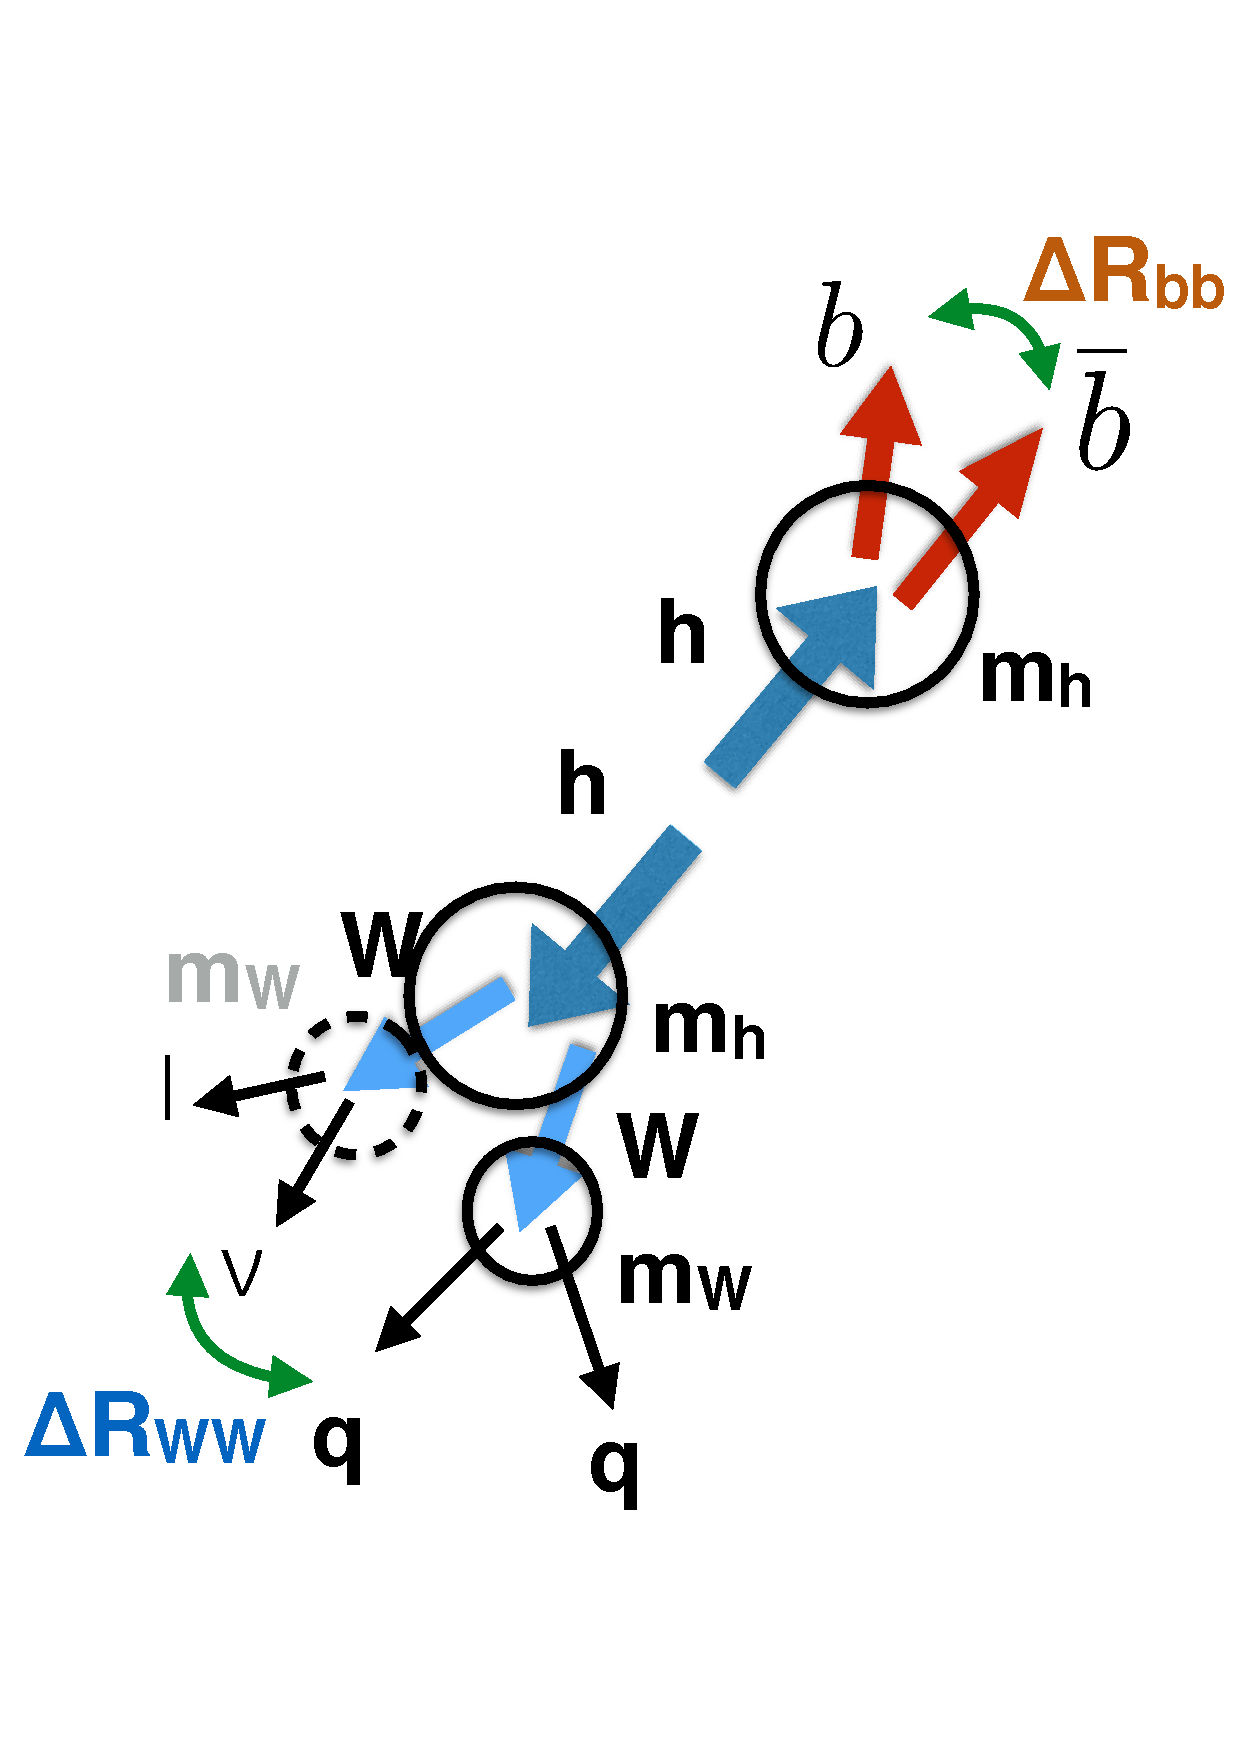
\includegraphics[width=0.4\textwidth]{figures/cartoon_hh.pdf}
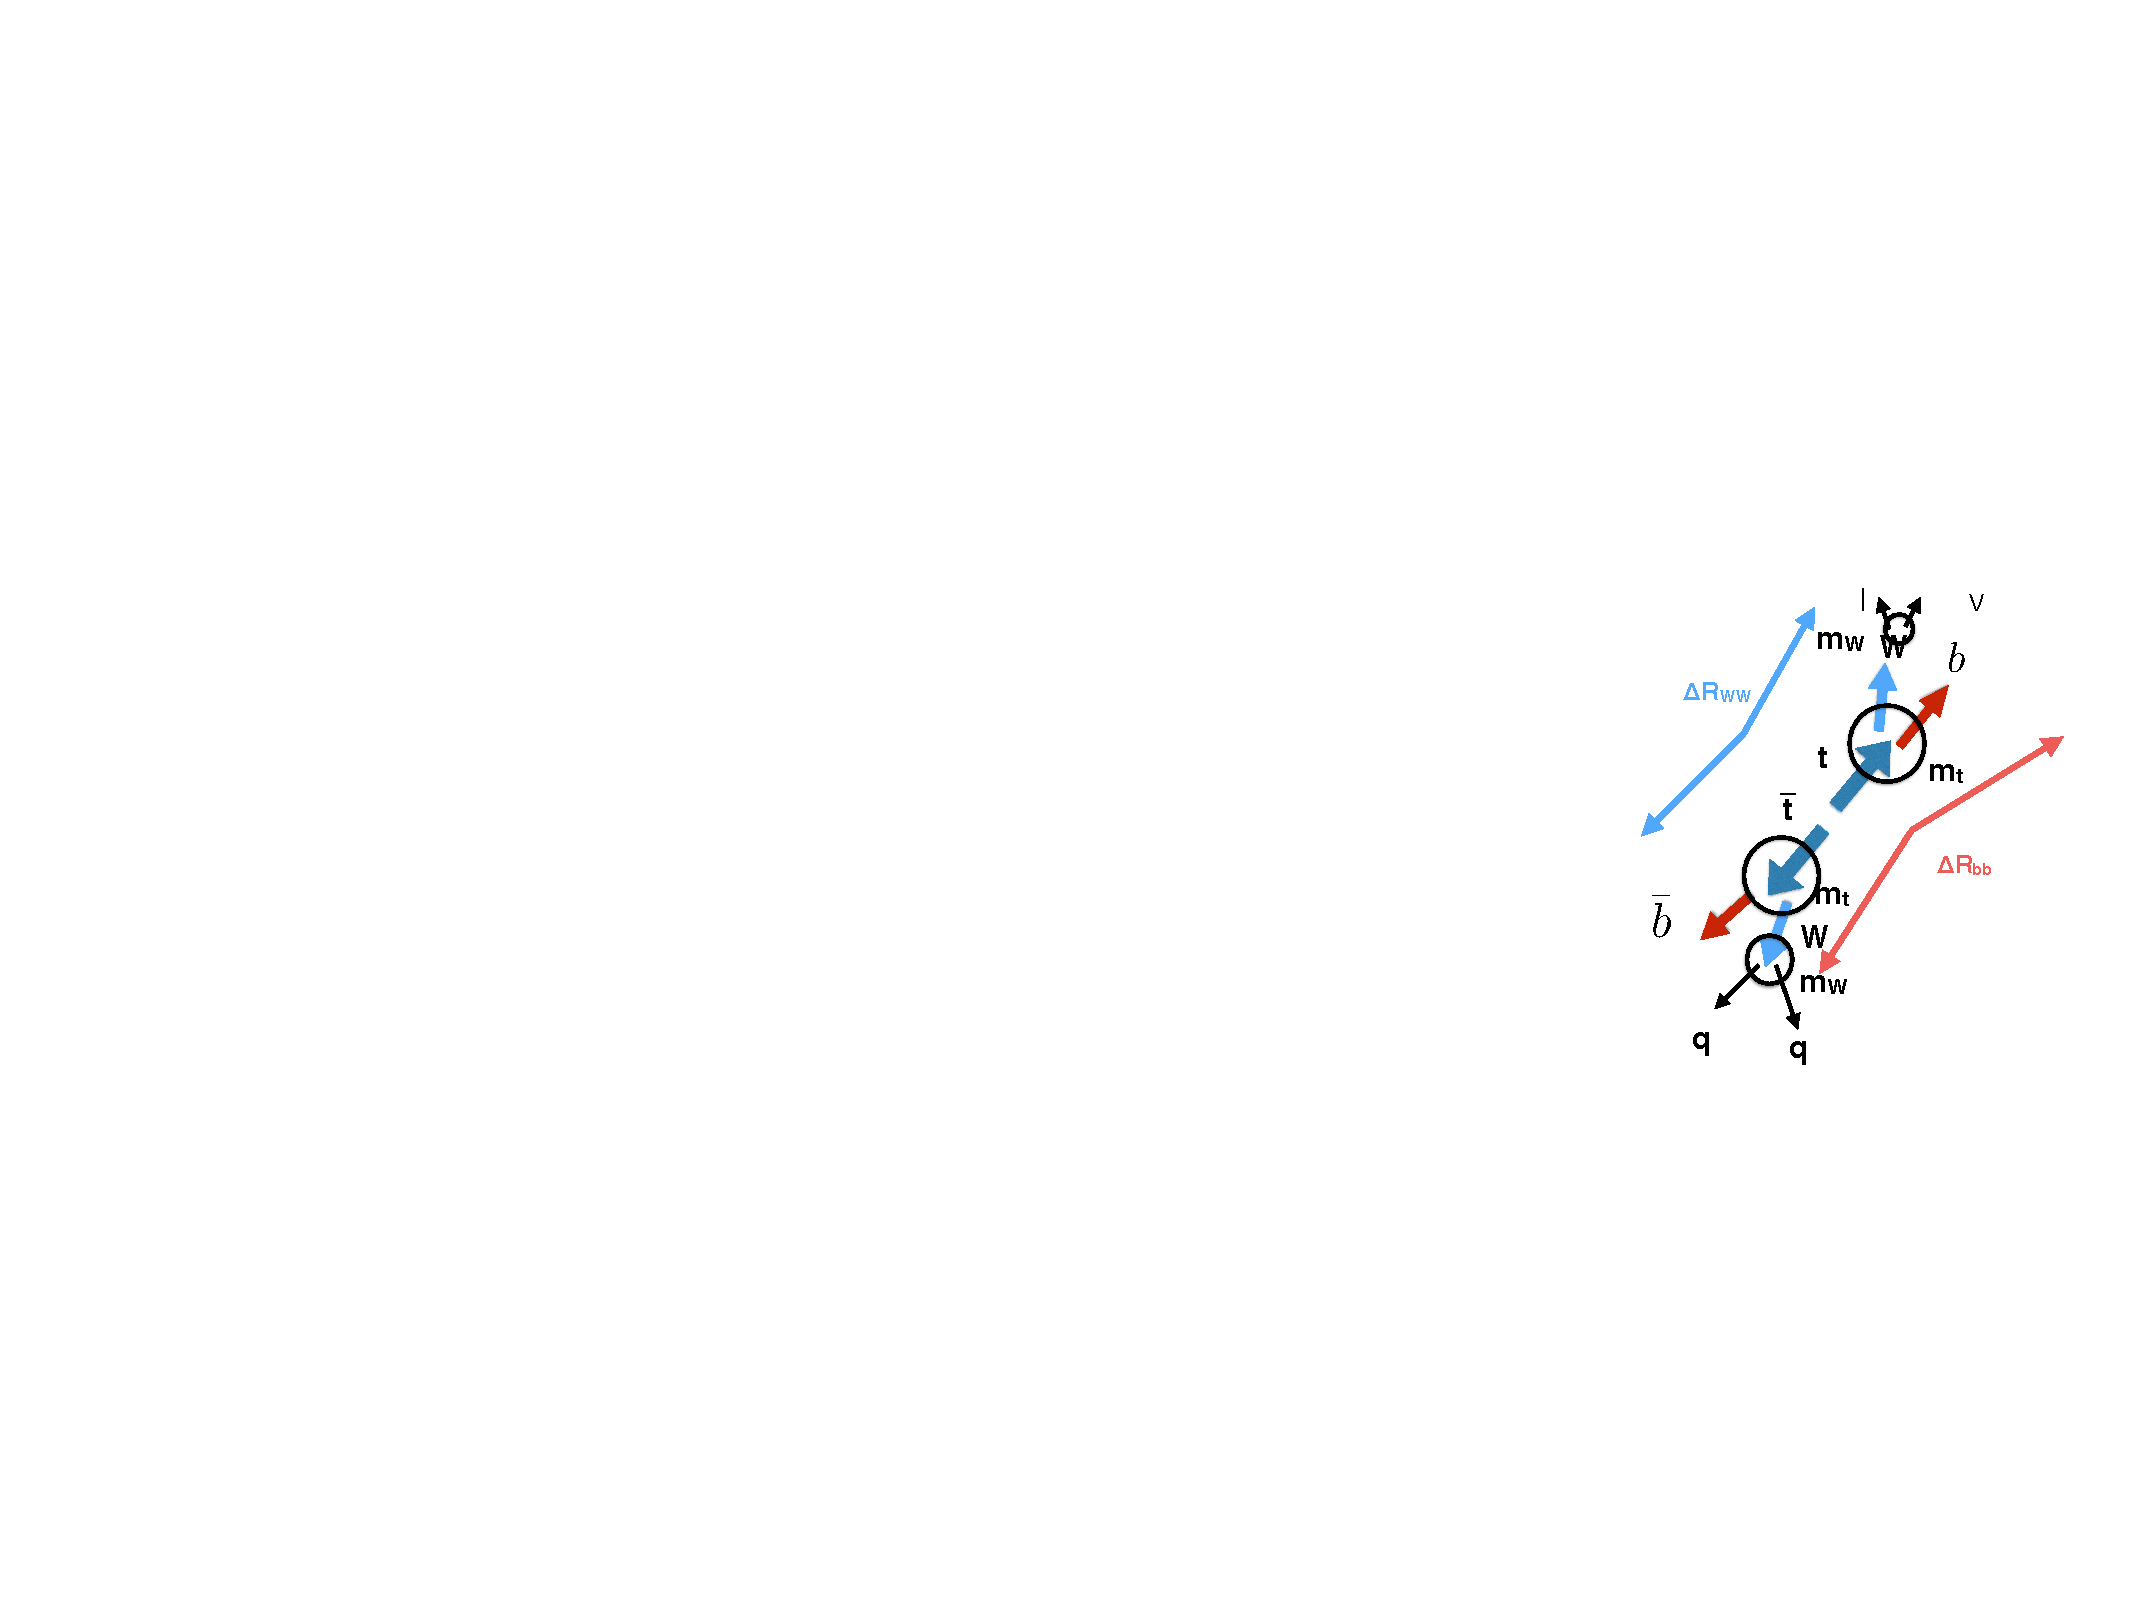
\includegraphics[width=0.4\textwidth]{figures/cartoon_tt.pdf}
\caption{Schematic view of a $HH \to WWbb$ event compared to a $t\bar{t} \to WWbb$ event.} 
\label{fig:cartoon}
\end{figure}

The $t \bar{t}$ events are typically characterised by two $b$-jets and
two $W$ bosons such that the $\Delta R$ separation between the two
$b$-jets and between the $W$ bosons is large. On the contrary, in particular
when the invariant mass of the $m_{HH}$ is high, the signal is characterised
by two $b$-jets which are close together in $\Delta R$ and by two $W$ bosons
which are also relatively closer than in the $t \bar{t}$
case. Moreover, while for the signal the two $b$-jets have an
invariant mass equal to $m_h$, this is not necessarily the case for the $t \bar{t}$ background.  Following these considerations, the typical separation variables are: 
\begin{itemize}
\item the $p_T$ of the $b \bar{b}$ pair ($p_T^{bb}$);
\item the $\Delta R$ of the $b \bar{b}$ pair ($\Delta R^{bb}$);
\item the $p_T$ of the $WW$ pair ($p_T^{WW}$);
\item the $\Delta R$ of the $WW$ pair ($\Delta R^{WW}$);
\item the mass of the $WW$ system computed using the calculated neutrino
      longitudinal momentum ($m_{\rm WW}$). This value is exactly equal to $m_h$
      if a real solution is found, it is larger if no real solution is found;
\item the invariant mass of the di-Higgs boson candidate system ($m_{HH}$). 
\item the invariant mass of the 2 b-jets boson system ($m_{bb}$). 

\end{itemize}


\subsection{Signal region definitions}
\label{subsec:SR}
The cuts of the selection have been optimised by maximising the Poisson
significance at the end of the selection \footnote{a two step procedure has
been implemented. In the first step each cut is optimised, in the second step,
all cuts are set to their optimal value and cuts are varied one by one to
look for a different optimisation point. Correlation among variables 
could in fact spoil the results obtained at the first step.}. The Poisson
significance formula depends on the absolute yield of expected signal and
background events. For the optimisation formula the \ttbar background was
normalised to data with $m_{bb} < 100$ GeV or $m_{bb} > 140$ GeV, 
such region rejects, in fact, the majority of the signal. Four signal
hypotheses have been used in the optimisation:
\begin{itemize}
\item{ a heavy Higgs with $m_H = 500$ GeV and $m_H = 700$ GeV (defined as low-mass analysis)},
\item{ a heavy Higgs with $m_H = 2000$ GeV (defined as high-mass analysis) and}
\item{ a non-resonant di-Higgs production (defined as non-resonant analysis).}
\end{itemize}
An additional mass point with $m_H = 1400$ GeV was also checked. The resulting selection and the corresponding sensitivity are very similar to the selection for $m_H = 2000$ GeV, and hence that selection is dropped.{\footnote {See \url {https://indico.cern.ch/event/641988/contributions/2604588/attachments/1465307/2265002/bbWW_Weekly_Optimization_Revisited_24May2018.pdf}}} 
%The signals have been normalised to the Run 1 upper limit scaled by the $13/8$ TeV cross section ratio expected from the
%PDF luminosity scale of a narrow resonance of that mass. 

The signal regions for the  reference signal hypotheses are summarised in 
Table~\ref{tab:sig_reg_summary}.


\begin{table}
\begin{center}
\begin{tabular}{c|c|c|c|c}
 variable & \emph{Non-Res} & \emph{m500} & \emph{low-mass} & \emph{high-mass}\\
\hline
$E^{\rm T}_{miss}$ (GeV)		&$> 25$&$>25$&$> 25$& $> 25$ \\
$m_{WW}$ (GeV) 	   		&$< 130$ &$< 130$ & $< 130$& no-cut\\
$p_{\rm T}^{bb}$ (GeV) 		&$> 300$& $> 210$&$> 210$&$> 350$\\
$p_{\rm T}^{WW}$ (GeV) 		&$> 250$&$> 150$&$> 250$&$> 250$ \\
$\Delta R_{WW}$  		&no-cut& no-cut&no-cut&$<1.5$\\
$m_{bb}$ (GeV)   		&105-135&105-135&105-135&105-135\\
\end{tabular}
\caption{Criteria for non-resonant, \emph{m500}, \emph{low-mass} and 
    \emph{high-mass} selection. The $m_{hh}$ window cut is not applied for 
    non-resonant signal, and for resonant signals $m_{hh}$ depends on 
    the mass.} 
\label{tab:sig_reg_summary}
\end{center}
\end{table}


The \textit{non-res} and \textit{m500} selections are exclusively used for non-resonant signal and resonant signal with mass 500 GeV respectively. The \textit{low-mass} selection is used for signal masses from 600 to 1300 GeV, while the \textit{high-mass} selection is used for signals with masses between 1400 and 3000 GeV. In addition, requirements are placed on the reconstructed di-Higgs invariant mass ${m_{HH}}$ as a function of the signal resonance mass ${m_{X}}$, as shown in Table \ref{tab:mhh_sig_cuts}. The resolution of the reconstructed mH H ranges from 6\% at 500 GeV to 10\% at 3000 GeV.

\begin{table}
\begin{center}
\begin{tabular}{c|c|c|c|c|c}
$m_{H}$ (GeV)      &   500   &   600   &   700   &   750   &   800 \\
$m_{hh}$ cut (GeV) & 480-530 & 560-640 & 625-775 & 660-840 & 695 - 905 \\ 
\hline 
$m_{H}$ (GeV)      &  900   &   1000  	   &  1100   	&  1200   		&   1300    \\
$m_{hh}$ cut (GeV) & 760-970	& 840-1160 & 925-1275	&1010-1390	&1095-1505  \\
\hline 
$m_{H}$ (GeV)      &   1400  		&  1500   		&  1600   		& 1800  		& 2000\\
$m_{hh}$ cut (GeV) &1250-1550	&1340-1660	&1430-1770	& 1750-2020 	& 1910-2170\\
\hline

\hline 
$m_{H}$ (GeV)      &   2250  		&  2500   		&  2750   		& 3000  		& \\
$m_{hh}$ cut (GeV) &2040-2460	&2330-2740	&2570-2950	& 2760-3210 	& \\
\end{tabular}
\caption{Window cuts on $m_{hh}$ as a function of the resonance mass
  $m_{H}$.}
\label{tab:mhh_sig_cuts}
\end{center}
\end{table}


\subsection{Background Determination}
In the present analysis we expect that at the end of the event selection the
sample will be largely dominated by $t \bar{t}$ and multi-jet background, therefore the $t\bar{t}$ background normalisation
is derived from data while, as described in Sec. \ref{sec:multijet}, the multi-jet
background is derived using a data-driven ABCD method.
For all the other backgrounds, e.g. di-boson, Higgs, $W$+jets, the
MC is used appropriately normalized by using the expected cross sections and the
integrated luminosity that has been collected.

\subsubsection{Top normalization and control region}
\label{subsec:topCR}
The \ttbar background is normalised and validated using  dedicated
control regions (CR). Three CR's are defined, one for the SR's of the non-resonant (CR1), one for the low-mass analysis (CR2), and one for the high-mass analysis (CR3).  The CRs are defined in Table \ref{tab:CRdef}.


Table \ref{tab:CR1} through \ref{tab:CR3} show the number of observed
events and expected background events in the top CRs, and also in the sideband across selections that serve as validation regions. The final signal region is defined by $m_{bb}$ cut of $105~\textrm{GeV} < m_{bb} < 135~\textrm{GeV}$ based on optimization. The sidebands are orthogonal to the SR by virtue of having the $m_{bb}$ cut reversed. $m_{bb} < 100$ GeV or $m_{bb} > 140$ GeV defines the sidebands in which the control regions are defined.  The 5 GeV buffer region is kept on both sides so as to be less affected by systematic effects at the edge. Fig.~\ref{fig:mbb_signal} shows $m_{bb}$ for various signal mass points. A comparative study of signal over background in these three regions shows that S/B in the final SR is 5 (20) times higher than in the sidebands for m2000 (non-resonance) while S/B in the final SR is approximate twice as high as in the buffer zones.  Table~\ref{tab:sigOverBkg} shows the ratios of S/B in the buffer zones and sidebands compared to the S/B in the final SR. 

\begin{figure}[!h]
\begin{center}
\includegraphics*[width=0.47\textwidth] {figures/bbMass_X500_X700_X1400_X2000_X3000.eps}
\caption[$m_{bb}$ resolution for signal and sum of backgrounds.]{$m_{bb}$ resolution for signal samples.}
\label{fig:mbb_signal}
\end{center}
\end{figure}

\begin{table}
\caption{The ratios of S/B in the buffer zone and sidebands compared to the S/B in the final SR. } 
\begin{center}
\begin{tabular}{c|c|c|c|c|}
Selection & non-res & m500 & m700 & m2000\\
\hline
Buffer/SR              	& 1.85 & 1.95  & 1.90 & 1.63\\
\hline
 Sidebands/SR	       & 20.5 & 12.6 & 13.4 & 5.6\\
\hline 
\end{tabular}
\label{tab:sigOverBkg}
\end{center}
\end{table}

\newpage
%%%%%%%%%%%%%%
\begin{table}
\caption{Definition of the kinematic regions used to normalise the Top background. $m_{bb} < 100$~GeV or $m_{bb} > 140~GeV$ defines the sidebands in which the control regions are defined. Expected SM backgrounds are then checked against data at each subsequent selection.} \label{tab:CRdef}
\begin{center}
%\begin{tabular}{c|c|c|c|c|cxs}
% variable 						& Non-Res 	 	& X700 		& X2000\\
%\hline
%$m_{WW}$ (GeV)   				& $<130$ 		   	&$<130$ 		& no-cut \\
%$p_{\rm T}^{bb}$ (GeV) 			& $>150$ 		  	& $>150$ 		&$>350$\\
%$\Delta R_{bb}$  				& no-cut 	 		& no-cut		& no-cut  \\
%$p_{\rm T}^{WW}$ (GeV) 			& no-cut	 	 	& no-cut   		& no-cut \\
%$\Delta R_{WW}$  				& no-cut 		 	& no-cut 		& no-cut \\
%$m_{hh}$ (GeV)  				& no-cut 			& no-cut 		& no-cut\\
%\hline
\begin{tabular}{c|c|c|c|}
 variable 						&CR1 				& CR2 	& CR3 \\
\hline					
$m_{bb}$ (GeV)						& $m_{bb} < 100$ or $m_{bb} > 140$ & $m_{bb} < 100$ or $m_{bb} > 140$ & $m_{bb} < 100$ or $m_{bb} > 140$\\
$m_{WW}$ (GeV)   				& $<130$ 		 		& $<130$		& no-cut \\
$p_{\rm T}^{bb}$ (GeV) 			& $>300$ 		 		& $>210$		&$>350$\\
\hline


\end{tabular}
\end{center}
\end{table}
%%%%%%%%%%%%%%%
\iffalse
\begin{table}
\caption{Definition of the kinematic regions used to normalise the Top background.} \label{tab:CRdef}
\begin{center}
\begin{tabular}{c|c}
\hline
\multicolumn{2}{c}{Top CR definitions} \\
\hline
non-res  &  ($m_{bb} < 100$ GeV or $m_{bb} > 140$ GeV ), $m_{WW} < 130$ GeV  and $p_T^{\rm bb} > 150$ GeV (to be edited) \\
low-mass &  ($m_{bb} < 100$ GeV or $m_{bb} > 140$ GeV ), $m_{WW} < 130$ GeV  and $p_T^{\rm bb} > 150$ GeV \\
high-mass &   ({$m_{bb} < 100$ GeV or $m_{bb} > 140$ GeV}) and $p_T^{\rm bb} > 350$ GeV \\
\hline
\end{tabular}
\end{center}
\end{table}
\fi
%%tables to be added yet


\newpage

\begin{center}
\begin{table}
\caption{ The number of observed
events and expected background events in the $m_{bb}$ side-bands for
the non-resonant selection. The top CR1 is defined at the bbpt300
selection. No NF has been applied to the background yields to show the level of data/expectation agreement before normalizing ttbar.  Only statistical uncertainties are shown.}
\begin{tabular}{l|c|c|c|c}
\hline\hline
\multicolumn{5}{c}{\textbf{CR1}: \mbb Sideband}\\\hline\hline
Sample  	& mww 	& bbpt210 	& bbpt300 	& wwpt250 	  \\\hline
\ttbar 	& 23776.6 $\pm$ 87.2 	& 531.7 $\pm$ 13.1 	& 109.9 $\pm$ 5.9 	& 63.9 $\pm$ 4.6 \\\hline 
QCD 	& 13310.5 $\pm$ 500.3 	& 250.2 $\pm$ 30.6 	& 33.7 $\pm$ 4.1 	& 21.4 $\pm$ 2.6	\\\hline 
W+jets 	& 3938.9 $\pm$ 31.1 	& 124.7 $\pm$ 3.5 	& 29.3 $\pm$ 1.4 	& 17.1 $\pm$ 1.1 	\\\hline 
SingleTop 	& 1605.4 $\pm$ 18.0 	& 76.0 $\pm$ 3.8 	& 20.1 $\pm$ 2.0 	& 13.5 $\pm$ 1.7\\\hline 
Dibosons 	& 109.9 $\pm$ 2.7 	& 8.3 $\pm$ 0.8 	& 2.2 $\pm$ 0.4 	& 1.5 $\pm$ 0.4 	\\\hline 
Z+jets 	& 1107.6 $\pm$ 8.4 	& 27.1 $\pm$ 0.8 	& 6.7 $\pm$ 0.4 	& 2.4 $\pm$ 0.2 	\\\hline 
\hline
Background Sum 	& 43849.0$\pm$ 509.2 	& 1017.9$\pm$ 33.7 	& 201.9$\pm$ 7.6 	& 119.8$\pm$ 5.7 \\\hline 
\hline
XhhSM 	& 44.6 $\pm$ 2.2 	& 9.1 $\pm$ 0.7 	& 1.5 $\pm$ 0.2 	& 1.1 $\pm$ 0.1 	\\\hline 
Data 	& 43902.0 	& 1069.0 	& 206.0 	& 138.0 \\\hline 
\hline
\end{tabular}
\label{tab:CR1}
\end{table}
\end{center}

\begin{center}
\begin{table}
\caption{ The number of observed
events and expected background events in the $m_{bb}$ side-bands for the low-mass selection, m500. The top CR2 is defined at the bbpt210 selection. To show how well the prediction matches data, no NF has been applied to any background. Only statistical uncertainties are shown.}
\begin{tabular}{l|c|c|c|c}
\hline\hline
\multicolumn{5}{c}{\textbf{CR2}: \mbb Sideband}\\\hline\hline
Sample  	& mww 	& bbpt210 	& wwpt150 	& hh500  \\\hline
\ttbar 	& 23776.6 $\pm$ 87.2 	& 531.7 $\pm$ 13.1 	& 432.7 $\pm$ 11.8 	& 35.5 $\pm$ 3.2 		\\\hline 
QCD 	& 13310.5 $\pm$ 500.3 	& 250.2 $\pm$ 30.6 	& 206.3 $\pm$ 25.3 	& 16.9 $\pm$ 2.1 		\\\hline 
W+jets 	& 3938.9 $\pm$ 31.1 	& 124.7 $\pm$ 3.5 	& 105.9 $\pm$ 3.3 	& 4.9 $\pm$ 0.6 	\\\hline 
SingleTop 	& 1605.4 $\pm$ 18.0 	& 76.0 $\pm$ 3.8 	& 64.9 $\pm$ 3.5 	& 2.8 $\pm$ 0.6 	\\\hline 
Dibosons 	& 109.9 $\pm$ 2.7 	& 8.3 $\pm$ 0.8 	& 6.7 $\pm$ 0.8 	& 0.9 $\pm$ 0.2 	\\\hline 
Z+jets 	& 1107.6 $\pm$ 8.4 	& 27.1 $\pm$ 0.8 	& 19.0 $\pm$ 0.7 	& 1.5 $\pm$ 0.2 		\\\hline 
\hline
Background Sum 	& 43849.0$\pm$ 509.2 	& 1017.9$\pm$ 33.7 	& 835.5$\pm$ 28.3 	& 62.5$\pm$ 3.9	\\\hline 
\hline
Xhh500 	& 3.2 $\pm$ 0.1 	& 0.6 $\pm$ 0.1 	& 0.6 $\pm$ 0.1 	& 0.2 $\pm$ 0.1 	\\\hline 
Data 	& 43902.0 	& 1069.0 	& 898.0 	& 73.0 	\\\hline 
\end{tabular}
\label{tab:CR2_500}
\end{table}
\end{center}
%%%%%%%%%%%%%%%%%
\begin{center}
\begin{table}
\caption{ The number of observed
events and expected background events in the $m_{bb}$ side-bands for the low-mass selection, m700. The top CR2 is defined at the bbpt210 selection. To show how well the prediction matches data, no NF has been applied to any background. Only statistical uncertainties are shown.}
\begin{tabular}{l|c|c|c|c}
\hline\hline
\multicolumn{5}{c}{\textbf{CR2}: \mbb Sideband}\\\hline\hline
Sample  	& mww 	& bbpt210 	& wwpt250 	& hh700   \\\hline
\ttbar 	& 23776.6 $\pm$ 87.2 	& 531.7 $\pm$ 13.1 	& 175.6 $\pm$ 7.5 	& 49.9 $\pm$ 3.9 	\\\hline 
QCD 	& 13310.5 $\pm$ 500.3 	& 250.2 $\pm$ 30.6 	& 72.4 $\pm$ 8.9 	& 28.4 $\pm$ 3.5 		\\\hline 
W+jets 	& 3938.9 $\pm$ 31.1 	& 124.7 $\pm$ 3.5 	& 45.7 $\pm$ 2.1 	& 13.7 $\pm$ 1.4 	\\\hline 
SingleTop 	& 1605.4 $\pm$ 18.0 	& 76.0 $\pm$ 3.8 	& 28.4 $\pm$ 2.4 	& 6.9 $\pm$ 1.1 		\\\hline 
Diboson 	& 109.9 $\pm$ 2.7 	& 8.3 $\pm$ 0.8 	& 2.8 $\pm$ 0.5 	& 0.7 $\pm$ 0.2 		\\\hline 
Z+jets 	& 1107.6 $\pm$ 8.4 	& 27.1 $\pm$ 0.8 	& 5.8 $\pm$ 0.4 	& 2.0 $\pm$ 0.3 		\\\hline 
\hline
Background Sum 	& 43849.0$\pm$ 509.2 	& 1017.9$\pm$ 33.7 	& 330.7$\pm$ 12.1 	& 101.5$\pm$ 5.5 	\\\hline 
\hline
Xhh700 	& 4.2 $\pm$ 0.2 	& 2.2 $\pm$ 0.1 	& 1.5 $\pm$ 0.1 	& 1.0 $\pm$ 0.1 	\\\hline 
Data 	& 43902.0 	& 1069.0 	& 367.0 	& 124.0	\\\hline 


\end{tabular}
\label{tab:CR2_700}
\end{table}
\end{center}
%%%%%%%%%%%%%%%%%%%
\begin{center}
\begin{table}
\caption{ The number of observed
events and expected background events in the $m_{bb}$ side-bands for
the high-mass selection. The top CR3 is defined at the bbpt350
selection. No NF has been applied to the background yields. Only statistical uncertainties are shown.}
\begin{center}
\begin{tabular}{l|c|c|c|c}
\hline\hline
\multicolumn{5}{c}{\textbf{CR3}: \mbb Sideband}\\\hline\hline
Sample  	& bbpt350 	& wwpt250 	& drww15 	& hh2000 	\\\hline
\ttbar 	& 8568.7 $\pm$ 52.1 	& 7095.6 $\pm$ 47.5 	& 1940.5 $\pm$ 25.1 	& 122.3 $\pm$ 6.5 \\\hline 
QCD 	& 1538.7 $\pm$ 252.7 	& 1359.5 $\pm$ 75.9 	& 392.7 $\pm$ 21.9 	& 20.7 $\pm$ 1.2 	\\\hline 
W+jets 	& 2259.5 $\pm$ 7.9 	& 1952.1 $\pm$ 7.4 	& 696.6 $\pm$ 4.6 	& 55.5 $\pm$ 1.1 	\\\hline 
SingleTop 	& 1778.1 $\pm$ 19.4 	& 1601.6 $\pm$ 18.4 	& 405.4 $\pm$ 9.2 	& 29.6 $\pm$ 2.6 	\\\hline 
Dibosons 	& 170.6 $\pm$ 3.9 	& 147.1 $\pm$ 3.7 	& 46.8 $\pm$ 2.1 	& 3.4 $\pm$ 0.6 	\\\hline 
Z+jets 	& 403.6 $\pm$ 2.1 	& 307.6 $\pm$ 1.8 	& 95.6 $\pm$ 1.1 	& 7.5 $\pm$ 0.3 	\\\hline 
\hline
Background Sum 	& 14719.1$\pm$ 258.9 	& 12463.5$\pm$ 91.8 	& 3577.5$\pm$ 35.0 	& 238.9$\pm$ 7.2	\\\hline 
\hline
Xhh2000 	& 25.7 $\pm$ 0.4 	& 24.0 $\pm$ 0.4 	& 9.6 $\pm$ 0.3 	& 2.9 $\pm$ 0.1	\\\hline 
Data 	& 14862.0 	& 12450.0 	& 3761.0 	& 250.0 	\\\hline 

\end{tabular}
\end{center}
\label{tab:CR3}
\end{table}
\end{center}

\begin{table}
\caption{Normalisation factors for the two CRs, the statistical error
  includes only data statistics, the systematic error is obtained
  subtracting in quadrature the statistical error from the total error.} \label{tab:NFs}
\begin{center}
\begin{tabular}{c|c|c|c}
\multicolumn{4}{c}{Top background normalisation factors in the two
  CRs.} \\
\hline
region & NF & $\sigma_{stat.}$ & $\sigma_{syst.}$ \\
\hline
non-res   & 1.04  &  $\pm$0.20  &  $\pm$0.43\\
low-mass  & 1.14  &  $\pm$0.10  &  $\pm$0.35\\
high-mass & 1.02  &  $\pm$0.02  &  $\pm$0.07\\
\hline
\end{tabular}
\end{center}
\end{table}

Table \ref{tab:CR1} through \ref{tab:CR3} show the number of observed
events and expected background events in the top CRs before the
normalisation factors have been applied to the top background sample.

The top normalisation factors are determined by a simultaneous fit  of
signal and control regions, which include both Top CR and QCD CR~\ref{sec:multijet}. It also depends slightly on the $m_{hh}$ window due to the presence of top background in the signal region, and it is furthermore different for the \emph{non  res}, \emph{low  mass} and \emph{high mass} analyses. The normalisation
factors of the three top control regions are shown in Table \ref{tab:NFs}.

Fig.~\ref{fig:mbb_mhh} shows the $m_{bb}$ and $m_{hh}$ distributions in the two CRs while in Appendix \ref{app:data_exp_reOptNonRes} through ~\ref{app:data_exp_reOpt2000} we show the complete distributions of the
relevant variables used in the analysis selection in the top CR.  

\begin{figure}[!h]
\begin{center}
\includegraphics*[width=0.47\textwidth] {figures/ControlPlots_new/reOptNonRes/C_reOptNonRes_mww_bbpt210_bbpt300_bbMass_regionA_met25d020}
\includegraphics*[width=0.47\textwidth] {figures/ControlPlots_new/reOptNonRes/C_mBBcr_reOptNonRes_mww_bbpt210_bbpt300_hhMass_regionA_met25d020}

\includegraphics*[width=0.47\textwidth] {figures/ControlPlots_new/reOpt700/C_reOpt700_mww_bbpt210_bbMass_regionA_met25d020}
\includegraphics*[width=0.47\textwidth] {figures/ControlPlots_new/reOpt700/C_mBBcr_reOpt700_mww_bbpt210_hhMass_regionA_met25d020}

\includegraphics*[width=0.47\textwidth] {figures/ControlPlots_new/reOpt2000/C_reOpt2000_bbpt350_bbMass_regionA_met25d020}
\includegraphics*[width=0.47\textwidth] {figures/ControlPlots_new/reOpt2000/C_mBBcr_reOpt2000_bbpt350_hhMass_regionA_met25d020}

\caption[$m_{bb}$ and $m_{hh}$ in CR1, CR2 and CR3.]{$m_{bb}$ and $m_{hh}$ in CR1, CR2 and CR3.  \ttbar NFs as described in~\ref{subsec:topCR} have been applied. The uncertainties shown include the statistical and systematic uncertainties described in ~\ref{sec:syst}. Data are blinded in the region $100 < m_{bb} < 140 $. }
\label{fig:mbb_mhh}
\end{center}
\end{figure}

\subsection{Multi-jet background}

\label{sec:multijet}
Multi-jet backgrounds can enter in the event selection if a jet from
heavy flavour decays is mis-identified as an electron or a muon and used
as a lepton in the analysis. Such phenomena are not accurately reproduced by MC
simulation, due to large uncertainties in the jet shower shape simulation
and uncertainties in muon fragmentation functions and kinematics. In order 
to estimate the contributions of multi-jet processes, a data-driven ABCD 
method is used to estimate this background in the present analysis.
%%Such methods are used extensively in the top group analyses.

The ABCD method uses three control regions (the B, C, and D regions) to estimate
the contribution of a given background in the signal (A) region. Cuts on two ideally
orthogonal variables are used to create the signal and various control regions, e.g. 
the A region passes both cuts, the B and C regions each pass one cut and fail the other, 
while the D region fails both cuts. The absolute value of the significance of the lepton 
impact parameter and the missing transverse energy (MET) are used as the two variables 
used to define the regions in the ABCD method for this analysis. The regions are thus 
defined 
\begin{itemize}
\item A region: MET $>$ 25 GeV, \dsig $<$ 2.0
\item B region: MET $<$ 25 GeV, \dsig $<$ 2.0
\item C region: MET $>$ 25 GeV, \dsig $>$ 2.0
\item D region: MET $<$ 25 GeV, \dsig $>$ 2.0
\end{itemize}
Figure~\ref{fig:abcdCartoon} shows a pictoral representation of the four regions.
\begin{figure}[h!]
\begin{center}
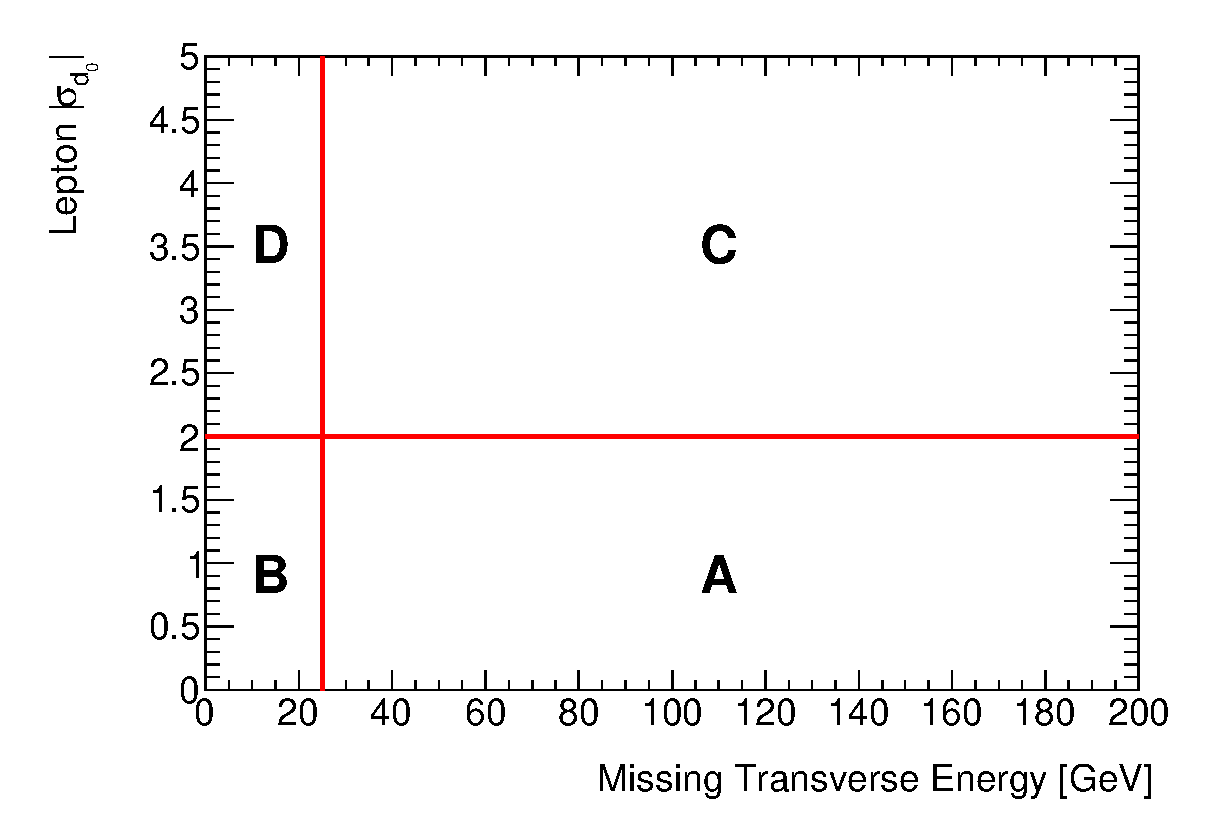
\includegraphics[width=0.6\textwidth]{figures/multijet/abcdExample_met_vs_d0sigBL20}
\end{center}
\caption{A pictoral representation of the four regions used in the
  ABCD calculation.} \label{fig:abcdCartoon}
\end{figure}
Assuming that the two variables chosen to define the ABCD regions are completely uncorrelated, the 
yield of the process being modelled (QCD multi-jets in this case) in the A region is given by
\begin{equation}
N_{A} = N_C \frac{N_B}{N_D}
\label{eq:simpleABCD}
\end{equation}
where the yields $N_i$ are yields calculated from data - all Monte Carlo backgrounds (\ttbar, 
W/Z+jets, single top, diboson processes) in region $i$ ($N_i = N_i^{\text{data}} - N_i^{\text{MC Bkgs}}$). 
The assumption underlying Equation~\ref{eq:simpleABCD} is that the relationship between the 
yields in the B and D regions is the same as the relationship between the A and C regions, i.e.
\begin{equation}
\frac{N_{A}}{N_{C}} = \frac{N_B}{N_D}
\label{eq:correlationStatement}
\end{equation}
Using equation ~\ref{eq:correlationStatement}, the quantity $R= \frac{N_{C} N_B}{N_{A} N_D}$ can be 
defined. In the case of two completely uncorrelated variables, $R=1$ and the ABCD estimation reduces 
to Equation~\ref{eq:simpleABCD}. If the two variables are not completely uncorrelated, the $R$ 
factor enters as a correction to Equation~\ref{eq:simpleABCD} for the multi-jet estimation in the A 
region, and the expression can be rewritten as
\begin{equation}
N_{A} = R \frac{N_C N_B}{N_D}
\label{eq:advancedABCD}
\end{equation}
The $R$ factor is calculated for each selection (non-resonant, low mass, and high mass) individually,
and the results at each cut in each selection is provided in
Table~\ref{tab:rValues}.


\begin{table}[h!]
\centering
\begin{tabular}{c|c|c|c}
\hline\hline
\multicolumn{4}{c}{QCD $R$ Values, Non-resonant Selection}\\\hline\hline
mww 	& bbpt210 	& bbpt300 	& wwpt250	\\\hline 
0.74 $\pm$ 0.04 	& 0.79 $\pm$ 0.23 	& 1.07 $\pm$ 1.18 	& ---	\\\hline \hline
%\end{tabular}

\multicolumn{4}{c}{QCD $R$ Values, Low Mass Selection (m500)}\\\hline\hline
mww 	& bbpt210 	& wwpt150 	& hh500	\\\hline 
0.74 $\pm$ 0.04 	& 0.79 $\pm$ 0.23 	& --- 	& ---	\\\hline \hline

%\begin{tabular}{c|c|c|c}
\multicolumn{4}{c}{QCD $R$ Values, Low Mass Selection (m700)}\\\hline\hline
mww 	& bbpt210 	& wwpt250 	& hh700	\\\hline 
0.74 $\pm$ 0.04 	& 0.79 $\pm$ 0.23 	& 0.09 $\pm$ 0.14 	& ---	\\\hline \hline
%\end{tabular}

%\begin{tabular}{c|c|c|c}
\multicolumn{4}{c}{QCD $R$ Values, High Mass Selection}\\\hline\hline
bbpt350 	& wwpt250 	& drww15 	& hh2000	\\\hline 
0.48 $\pm$ 0.09 	& 0.43 $\pm$ 0.08 	& 0.50 $\pm$ 0.16 	& 4.28 $\pm$ 5.30	\\\hline 
\hline\hline
\end{tabular}


\caption{Values calculated for $R$ at each stage in the non-resonant,
  low mass, and high mass selections. The estimate of multi-jet
  contribution in the A region uses the $R$ value calculated after the
  first cut of each selection.} \label{tab:rValues}
\end{table}
In order to minimize the statistical error on $R$, the $R$ value calculated after 
the first cut of each selection (0.74 and 0.48) is used in Equation~\ref{eq:advancedABCD} to estimate the multi-jet
background after each subsequent cut. This can be done given the
compatibility of the $R$ value at the end of the cut flow with that at
the point where $R$ is evaluated. In order to check such compatibility
with higher statistics, the $R$ value has been calculated applying
each selection cut just after the cut where $R$ is evaluated, in order
to check that $R$ is not correlated with each of the selection cuts.
The result is shown in Table \ref{tab:R_after_X}.

\begin{table}[h!]
\centering

\begin{tabular}{c|c|c|c}
\hline\hline

%\multicolumn{2}{c}{QCD $R$ Values, Non-resonant Selection}\\\hline\hline
%mww 	                & mww + bbpt210 	\\\hline 
%0.74 $\pm$ 0.04 	& 0.79 $\pm$ 0.23 	\\\hline \hline
%\multicolumn{2}{c}{QCD $R$ Values, Low Mass Selection}\\\hline\hline
%mww 	                & mww + bbpt210 	\\\hline 
%0.74 $\pm$ 0.04 	& 0.79 $\pm$ 0.23 	  \\\hline \hline
%\multicolumn{2}{c}{QCD $R$ Values, High Mass Selection}\\\hline\hline
%bbpt350 	        & bbpt350 + wwpt250 	\\\hline 
%0.48 $\pm$ 0.09 	& 0.43 $\pm$ 0.08 	\\\hline 


\multicolumn{4}{c}{QCD $R$ Values, Non-resonant Selection}\\\hline\hline
mww 	                & mww + bbpt210 	& mww + bbpt300 	& mww + wwpt250 	\\\hline 
0.74 $\pm$ 0.04 	& 0.79 $\pm$ 0.23 	& 1.12 $\pm$ 1.22 	& 0.25 $\pm$ 0.20 	\\\hline \hline
\multicolumn{4}{c}{QCD $R$ Values, Low Mass (m500) Selection}\\\hline\hline
mww 	                & mww + bbpt210 	& mww + wwpt150 	& mww + hh500	  \\\hline 
0.74 $\pm$ 0.04 	& 0.79 $\pm$ 0.23 	& 0.50 $\pm$ 0.08 	& 0.52 $\pm$ 0.09  \\\hline \hline
\multicolumn{4}{c}{QCD $R$ Values, Low Mass (m700) Selection}\\\hline\hline
mww 	                & mww + bbpt210 	& mww + wwpt250 	& mww + hh700	  \\\hline 
0.74 $\pm$ 0.04 	& 0.79 $\pm$ 0.23 	& 0.25 $\pm$ 0.20 	& 0.63 $\pm$ 0.13  \\\hline \hline
\multicolumn{4}{c}{QCD $R$ Values, High Mass Selection}\\\hline\hline
bbpt350 	        & bbpt350 + wwpt250 	& bbpt350 + drww15 	& bbpt350 + hh2000	\\\hline 
0.47 $\pm$ 0.06 	& 0.44 $\pm$ 0.08 	& 0.52 $\pm$ 0.17	& 1.07 $\pm$ 0.67 	\\\hline 

\hline\hline
\end{tabular}

\caption{Values of $R$ obtained applying a single selection cut after the cut stage where $R$ is nominally evaluated.} \label{tab:R_after_X}
\end{table}


Once the normalization of the multi-jet background in the A region is calculated using Equation~\ref{eq:advancedABCD}, the shape of the multi-jet template is taken from the data - Monte Carlo distribution in the C region since the two are kinematically identical except for the cut on \dsig.

The uncertainty due to the limited statistics in the B and D regions is the
main source of the multi-jet estimation method systematics. In order to minimise
such error,  the yields from the  B and D regions used in the ABCD
calculation are frozen at a level of the cutflow to minimise statistical fluctuations.
The B and D region yields are frozen after the \ptbb $>$ 210 GeV cut for the non-resonant and low mass selection, and after the $p_{T}(WW)>$ 250 GeV for the high mass selection. Appendix~\ref{app:qcd_BDregionStudy_appendix} details the study carried out to select the stage at which to freeze the B and D regions. 

To further reduce the error coming from the C region, the shape of the data - Monte Carlo, i.e. non-prompt, 
\mbb distribution was studied as a function of each individual cut for each selection. If the \mbb shape is 
unchanged by the additions of cuts later in a given selection, the C region shape can be taken from an 
earlier stage in the cutflow, reducing the shape uncertainty and overall statistical error on the QCD yield.
To determine the stability of the \mbb shape, the ratio of events in the \mbb signal region ([100, 140] GeV)
over the numbers of events in the full \mbb spectrum was computed for each individual cut using the C region 
of the ABCD method. This ratio was found to be stable across each selection, and the results of this 
calculation are provided in Table~\ref{tab:efficiencyFactor}. 

  \begin{table}[h!]%\fontsize{8}{9}\selectfont
    \centering
    \begin{tabular}{c|c|c|c}
      \hline\hline
      \multicolumn{4}{c}{reOptNonRes: \mbb SR/Total Ratios For Individual Cuts}\\\hline\hline 
      mww 	& bbpt210 	& bbpt300 	& wwpt250 	\\\hline 
      0.17 $\pm$ 0.02 	& 0.15 $\pm$ 0.03 	& 0.13 $\pm$ 0.05 	& 0.16 $\pm$ 0.05 	\\\hline 
    \end{tabular}
    \vspace{5pt}
    
    \begin{tabular}{c|c|c|c}
      \hline\hline
      \multicolumn{4}{c}{reOpt500: \mbb SR/CR Ratios For Individual Cuts}\\\hline\hline 
      mww 	& bbpt210 	& wwpt150 	& hh500 	\\\hline 
      0.17 $\pm$ 0.02 	& 0.15 $\pm$ 0.03 	& 0.18 $\pm$ 0.02 	& 0.22 $\pm$ 0.03 	\\\hline 
    \end{tabular}
    \vspace{5pt}

    \begin{tabular}{c|c|c|c}
      \hline\hline
      \multicolumn{4}{c}{reOpt700: \mbb SR/Total Ratios For Individual Cuts}\\\hline\hline 
      mww 	& bbpt210 	& wwpt250 	& hh700 	\\\hline 
      0.17 $\pm$ 0.02 	& 0.15 $\pm$ 0.03 	& 0.16 $\pm$ 0.05 	& 0.16 $\pm$ 0.02 	\\\hline 
    \end{tabular}
    \vspace{5pt}

    \begin{tabular}{c|c|c|c}
      \hline\hline
      \multicolumn{4}{c}{reOpt2000: \mbb SR/Total Ratios For Individual Cuts}\\\hline\hline 
      bbpt350 	& wwpt250 	& drww15 	& hh2000 	\\\hline 
      0.12 $\pm$ 0.08 	& 0.16 $\pm$ 0.05 	& 0.19 $\pm$ 0.02 	& 0.11 $\pm$ 0.14 	\\\hline 
      \hline 
    \end{tabular}
    \caption{The ratio of events in the \mbb signal region ([100, 140] GeV) over the numbers of events in the full \mbb spectrum for each individual cut. Both event yields are calculated in the C region of the ABCD method. The ratios are found to be stable across each selection.}        \label{tab:efficiencyFactor}
  \end{table}

The normalized shapes of the full \mbb distributions after each 
cut are shown in Figure~\ref{fig:mbbShapes}. The earliest selection cut with a consistent shape was chosen as the
shape for each cutflow and this corresponds to the shape obtained
after the  \ptbb $>$ 210 GeV cut 
for the non-resonant the m500 and m700  selections,  and after the  \ptww $>$ 250 GeV for the m2000 selection.



\subsection{Signal Region plots and Cutflow}
\subsection{Systematic Uncertainties}





\section{Boosted Analysis}
\subsection{Event Selection}
\subsection{Background Determination}
\subsection{Systematic Uncertainties}
\section{Results}
\subsection{Resolved Analysis}
\subsection{Boosted Analysis}
\section{Summary}
\section{Conclusion}


